%------------------------------------------------------------------------------------
%	CHAPTER 6
%------------------------------------------------------------------------------------
\chapterimage{headConceito.png}
\chapter{Modelos Complementares}

\begin{remark}
Há verdadeiramente duas coisas diferentes: saber e crer que se sabe. A ciência consiste em saber; em crer que se sabe reside a ignorância. (Hipócrates - Filosofo Grego e Pai da Medicina) 
\end{remark}

\section{DBScan}\index{Modelos Complementares}
Todos os modelos vistos anteriormente são com certeza os mais utilizados, porém nem por isso são os únicos. Nesse último capítulo vamos investigar os modelos, digamos, não tão comuns mas que podem ser classificados como Complementares, não imagine que são largados ao acaso ou que podem ser esquecidos.

Esse é o mais contraditório dos modelos, calma que me explico. O nome \textit{DBScan} parece bem curto, mas é apenas uma sigla para \textit{Density-Based Spatial Clustering of Applications with Noise}. É um algorítimo não supervisionado destinado a clusterização que é excelente para identificar \textit{outliers}.

Basicamente esse modelo trabalha com duas informações: EPS é a distância máxima entre 2 amostras para formar um cluster de mesmo tipo (neighborhood). minPts é o número mínimo de uma amostra na vizinhança para ser classificada como "\textit{Core Point}" (um pouco acima que os minPts na EPS). E nesse ponto entra em cena um \textit{noise} (traduzido literalmente para ruído ou barulho incômodo) e que para nós será tudo o que não for um \textit{Core Point} ou \textit{Border Point} (que são pontos um pouco abaixo que os minPts na EPS).

Esquecendo esse negócio de conceito, vejamos como isso funciona na prática, utilizamos a base Íris pois será bem mais fácil quando já conhecemos bem os dados. Ativamos nosso JupyterLab personalizado que criamos com o Docker e na primeira célula importamos as bibliotecas necessárias:
\begin{lstlisting}[]
import pandas as pd
import numpy as np
from sklearn import datasets
from sklearn.cluster import DBSCAN
from matplotlib import pyplot as plt
from sklearn.datasets import make_moons

%matplotlib inline
\end{lstlisting}

As bibliotecas são Pandas e NumPy para organizar nossos dados, da Scikit-Learn vamos trazer os dados pela datasets e o algorítimo pela DBSCAN e a MatPlotLib para mostrá-los de modo gráfico.

\section{Explicação do noise}\index{Modelos Complementares}
Antes de começarmos precisamos entender bem como ocorre um "distúrbio nos dados", para isso usaremos a base \textit{make\_moons} para produzir alguns dados:
\begin{lstlisting}[]
X, label = make_moons(n_samples=200, noise=0.01)
X[0:5]
\end{lstlisting}

O mais importante aqui é observamos o parâmetro \textit{noise}. Começamos com um valor bem baixo, ou seja, quase nenhum ruído será produzido nos dados. Identificamos uma variável label que corresponde a resposta dos dados, e é nela que devemos ficar atentos, verificamos seu valor:
\begin{lstlisting}[]
print(label)
\end{lstlisting}

E observamos que basicamente temos uma série de 0s e 1s, isso indica que os dados contém 2 clusters. Ao treinarmos nosso modelo:
\begin{lstlisting}[]
model = DBSCAN(eps=0.25, min_samples=10)
model.fit(X)
\end{lstlisting}

Descobriremos que ao visualizarmos os \textit{labels}:
\begin{lstlisting}[]
print(model.labels_)
\end{lstlisting}

O resultado da variável resposta é igual ao original, mas isso fica mais claro se visualizarmos de forma gráfica, então:
\begin{lstlisting}[]
# Original
fig, ax = plt.subplots(figsize=(6,5))
ax.scatter(X[:,0], X[:,1], c=label)
fig.show()

# Predito
fig, ax = plt.subplots(figsize=(6,5))
ax.scatter(X[:,0], X[:,1], c=model.labels_)
fig.show()
\end{lstlisting}

E temos o seguinte resultado:
\begin{figure}[H]
	\centering
	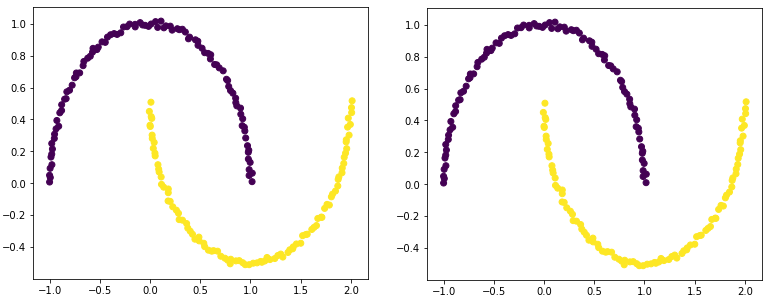
\includegraphics[width=0.6\textwidth]{cap06/dbscan1}
	\caption{Visualização dos Resultados em Noise com 0,01}
\end{figure}

Observamos que são duas curvas iguais (não se preocupe pois as cores podem variar) o importante nesse desenho é repararmos dois detalhes: primeiro são 2 clusters de dados e os pontos estão bem próximos.

A medida que aumentamos o parâmetro noise, os pontos vão se afastando (façamos alguns teste e aumentando gradativamente). Ao chegarmos no valor 0,1 temos a seguinte situação:
\begin{figure}[H]
	\centering
	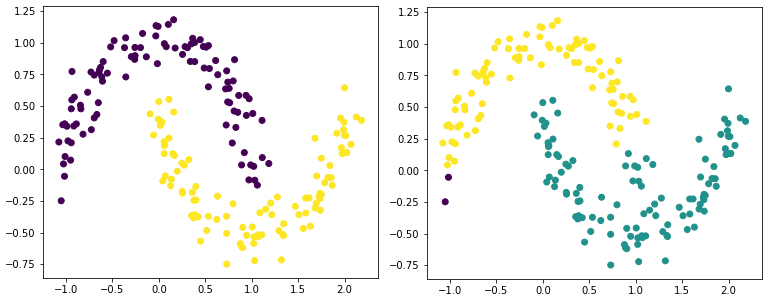
\includegraphics[width=0.6\textwidth]{cap06/dbscan2}
	\caption{Visualização dos Resultados em Noise com 0,1}
\end{figure}

E é essa imagem que buscamos, pois ao invés de 2 clusters foi predito um 3, e esse terceiro é formado por dois pontos (no segundo gráfico em roxo). Ou seja, foi lançado tanto ruído que o modelo se atrapalhou. Além disso, ao olharmos a variável model.labels\_ veremos que existem valores -1.

\section{Atrás dos outliers da Íris}\index{Modelos Complementares}
Agora que já sabemos o que é um ruído podemos voltar para a base Íris. Inicialmente carregamos a base de dados:
\begin{lstlisting}[]
iris = datasets.load_iris()
df = pd.DataFrame(data=np.c_[iris['data'], iris['target']], 
columns=iris['feature_names'] + ['Species'])
df.head()
\end{lstlisting}

Agora precisamos treinar o modelo:
\begin{lstlisting}[]
model = DBSCAN(eps=0.8, min_samples=19).fit(df)
print(model)
\end{lstlisting}

Porque 0,8 no EPS? Simples tentativa e erro, assim com o número mínimo de amostras em 19, não existe uma regra aplicável a qualquer base. Esse é um dos trabalhos em ser um Cientista de Dados. Apenas para facilitar, vamos pegar a fatia de dados que são suspeitas de outliers:
\begin{lstlisting}[]
df[model.labels_==-1]
\end{lstlisting}

E descobrimos que nessa situação temos 7 pontos suspeitos de serem outliers. Colocando-os em um gráfico:
\begin{lstlisting}[]
fig = plt.figure()
ax = fig.add_axes([.1, .1, 1, 1])
colors = model.labels_
ax.scatter(df.iloc[:,2], df.iloc[:,1], c=colors, s=120)
ax.set_xlabel('Tam Pétala')
ax.set_ylabel('Lrg Sépala')
plt.title('DBSCAN para Detecção de Outliers')
plt.show()
\end{lstlisting}

Temos o seguinte resultado:
\begin{figure}[H]
	\centering
	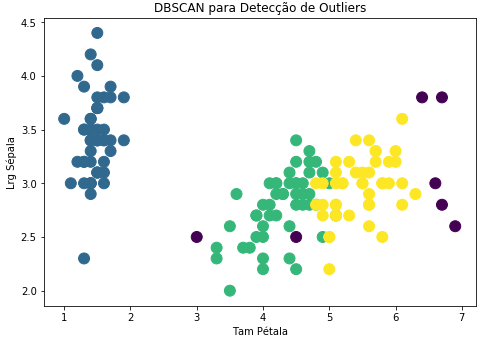
\includegraphics[width=0.5\textwidth]{cap06/dbscan3}
	\caption{Visualização dos Outliers da Iris}
\end{figure}

Agora já temos a faca e o queijo na mão, devemos lembrar da nossa primeira forma de descobrir \textit{outliers} (usando BoxPlots) não foi muito bem sucedida com o modelo KNN, talvez com alguns desses pontos conseguimos verificar se as espécies são realmente coerentes segundo nosso classificador.

\clearpage
